\clearpage\chapter{Inverse Functions}
Inverse functions are a direct extention of composite functions because the definition is derived from it. Let's learn how to find an inverse of a function.

To find the inverse of a function, simply rewrite the function as an equation of $y$, swap the $x$ and $y$, and solve for $y$. That's about it. Let's try it with an example.

\begin{problem}
    Given the function $f(x) = 3x^2$, find it's inverse.
\end{problem}
\begin{solution}
    We're given the function $f(x) = 3x^2$. First, we'll rewrite it as an equation of $y$.
    \[
        y = 3x^2
    \]
    Then, we'll swap the $x$ and $y$.
    \[
    x = 3y^2
    \]
    Finally, we'll solve for $y$.
    \begin{align*}
    x &= 3y^2 \\
    \frac{x}{3} &= y^2 \\
    \sqrt{\frac{x}{3}} &= y
    \end{align*}
    We can now rewrite this as the inverse function of $f$.
    \[
    f^{-1}(x) = \sqrt{\frac{x}{3}}
    \]
\end{solution}
Notice how the graphs of $f$ (blue) and $f^{-1}$ (red) intersect in the first quadrant of the $xy$-plane.
\begin{center}
    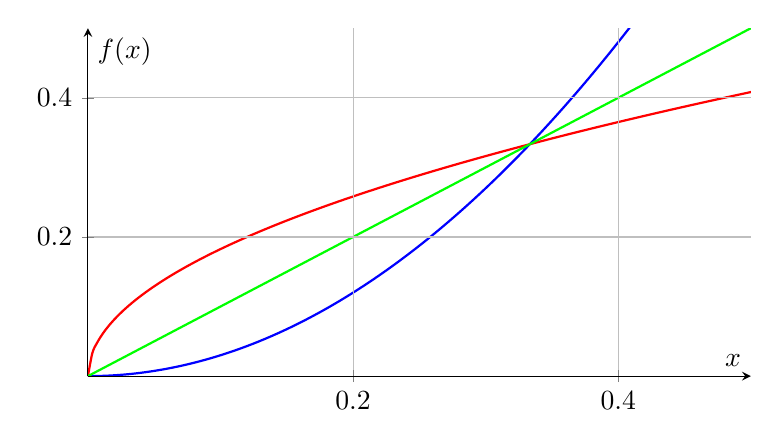
\begin{tikzpicture}
        \begin{axis}[
            axis lines = middle,
            xlabel = $x$, ylabel = {$f(x)$},
            xmin = 0, xmax = 0.5,
            ymin = 0, ymax = 0.5,
            xtick distance={0.2}, ytick distance={0.2},
            grid = both,
            width = 10cm,
            height = 6cm,
            samples = 10,
            smooth,
            axis on top,
        ]
        \addplot[blue, thick, domain=0:1, samples=300] {3*x^2};
        \addplot[red, thick, domain=0:1, samples=300] {sqrt(x / 3)};
        \addplot[green, thick, domain=0:1, samples=300] {x};
        \end{axis}
    \end{tikzpicture}
\end{center}
They are symmetrical along the line $y = x$ (green). Creating a table for each of these functions side by side reveals yet another property that inverse functions have.

Let's substitute $x = 3$ into $f$. That gives:
\begin{align*}
    f(3) &= 3(3)^2 \\
    &= 3(9) \\
    &= 27
\end{align*}
Now, let's plug this value into the inverse function $f^{-1}$.
\begin{align*}
    f^{-1}(3) &= \sqrt{\frac{27}{3}} \\
    &= \sqrt{9} \\
    &= 3
\end{align*}
Let's try the same for a different value, like $5$.
\begin{align*}
    f(5) &= 3(5)^2 & f^{-1}(75) &= \sqrt{\frac{75}{3}} \\
    &= 3(25) & &= \sqrt{25} \\
    &= 75 & &= 5
\end{align*}
What this means is: plugging the $y$-value of $f$ into $f^{-1}$ gives the $x$ value of $f$. A cleaner way of demonstrating this is by creating tables of each function side by side.
\begin{center}
    \begin{tabular}{ c | c }
        $x$ & $f(x) = 3x^2$ \\
        \hline
        $1$ & $3$ \\
        \hline
        $2$ & $12$ \\
        \hline
        $3$ & $27$
    \end{tabular}
    \quad
    \begin{tabular}{ c | c }
        $x$ & $f^{-1}(x) = \sqrt{\frac{x}{3}}$ \\
        \hline
        $3$ & $1$ \\
        \hline
        $12$ & $2$ \\
        \hline
        $27$ & $3$
    \end{tabular}
\end{center}
You may have noticed at this point that I haven't included the left side of the parabola. That's because the left side is \textbf{not} actually part of the inverse. The inverse function $f^{-1} = \sqrt{\frac{x}{3}}$ is a radical, meaning the result of $f^{-1}$ are valid. If I use negative $x$ values for $f$, I literally cannot swap the $x$ and $y$. The $x$ in $f(x)$ is being square, which negates any negative.
\begin{center}
    \begin{tabular}{ c | c }
        $x$ & $f(x) = 3x^2$ \\
        \hline
        $-1$ & $3$ \\
        \hline
        $-2$ & $12$ \\
        \hline
        $-3$ & $27$
    \end{tabular}
    \quad
    \begin{tabular}{ c | c }
        $x$ & $f^{-1}(x) = \sqrt{\frac{x}{3}}$ \\
        \hline
        $3$ & $1$ (not negative!!) \\
        \hline
        $12$ & $2$ (not negative!!)\\
        \hline
        $27$ & $3$ (not negative!!)
    \end{tabular}
\end{center}\clearpage
If I include the left side of the parabola in the graph I presented before, you can see why this is true.
\begin{figure}[ht]
    \caption{Parabola-Radical Example}
    \label{fig:Parabola-Radical Example}
    \centering
    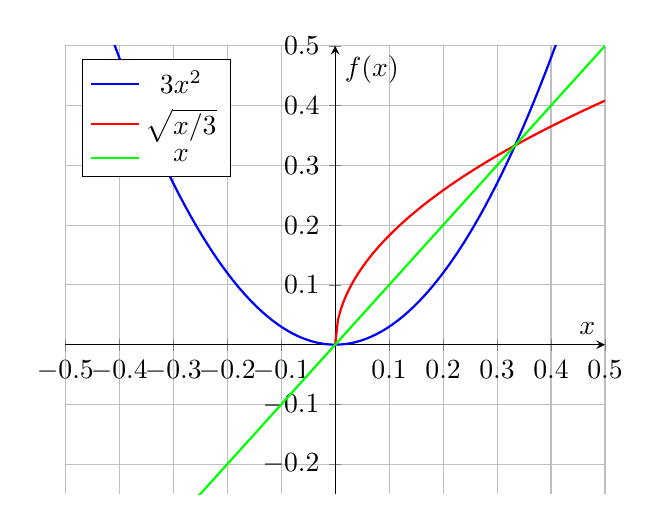
\begin{tikzpicture}
        \begin{axis}[
            axis lines = middle,
            xlabel = $x$, ylabel = {$f(x)$},
            xmin = -0.5, xmax = 0.5,
            ymin = -0.25, ymax = 0.5,
            xtick distance={0.1}, ytick distance={0.1},
            grid = both,
            legend pos = north west, % Positions the legend
        ]
            \addplot[blue, thick, domain=-0.5:0.5, samples=100] {3*x^2};
            \addlegendentry{$3x^2$}

            \addplot[red, thick, domain=0:0.5, samples=100] {sqrt(x / 3)};
            \addlegendentry{$\sqrt{x/3}$}

            \addplot[green, thick, domain=-0.5:0.5, samples=100] {x};
            \addlegendentry{$x$}
        \end{axis}
    \end{tikzpicture}
\end{figure}

The function $f^{-1}$ (red line) does not intersect $f$ (blue line) \textbf{or} $y = x$ (green line) when $x < 0$.

Let's formalize this with a definition.
\begin{definition}
    Given a function $f$, it's inverse $f^{-1}$ is such that
    \[
        f(f^{-1}) = x \text{ and } f^{-1}(f(x)) = x
    \]
    and the domain of $f$ is equal to the range of $f^{-1}$ (and vise versa).
\end{definition}
\clearpage
Before giving a problem for you to try on your own, I'll solve one more, slightly more difficult problem.

Given the function $f(x) = 3x^2 + 2x - 1$, find its inverse $f^{-1}$ and state its domain.

First, I'll rewrite it as an equation of $y$ and swap the variables
\begin{align*}
    y &= 3x^2 + 2x - 1 \\
    x &= 3y^2 + 2y - 1
\end{align*}
Now I'll solve for $y$.
\begin{align*}
    0 &= 3y^2 + 2x - 1 - x \\
    0 &= 3y^2 + 2x - (1 + x)
\end{align*}
I'll use the quadratic formula on the above equation with $a$, $b$, and $c$ defined like so
\[
\begin{aligned}
    a &= 3 \\
    b &= 2 \\
    c &= -(1 + x) = -x - 1
\end{aligned}
\]
The reason I'm using the quadratic formula is because we're given the standard form of a quadratic: $ax^2 + bx + c$. In the same way you'd solve for $x$ by using the quadratic formula, we can solve for $y$ using the quadratic formula. The solution for $y$ is as follows.
\begin{align*}
y &= \frac{-(2) \pm \sqrt{(2)^2 - 4(3)(-x - 1)}}{2(3)} && \text{Applied Quadratic Formula}\\
&= \frac{-2 \pm \sqrt{4 + 12(x + 1)}}{6} && \text{Simplified Radicand and Denominator}\\
&= \frac{-2 \pm \sqrt{4 + 12x + 12}}{6} && \text{Distributed $12$ Into The Parentheses}\\
&= \frac{-2 \pm \sqrt{12x + 16}}{6} && \text{Added Like Terms}\\
&= \frac{-2 \pm \sqrt{4(3x + 4)}}{6} && \text{Factored Out $4$ (the perfect square)}\\
&= \frac{-2 \pm 2\sqrt{3x + 4}}{6} && \text{Took $\sqrt{4} = 2$}\\
&= \frac{-1 \pm \sqrt{3x + 4}}{3} && \text{Divided Top and Bottom By $2$}
\end{align*}
\[
y = \frac{-1 \pm \sqrt{3x + 4}}{3} 
\]
In this case, we're only interested in the positive solution for $y$ for a few reasons:
\begin{enumerate}
    \item We want to ensure that the resulting expression is actually a function. Leaving it as $\pm$ turns the parabola sideways, which fails the vertical line test.
    \item The negative solution introduces a complication that I'll explain in just a moment.
\end{enumerate}
That leaves us with this inverse function as our solution.
\[
\boxed{f^{-1}(x) = \frac{\sqrt{3x + 4} - 1}{3}} \qquad \text{Swapped the terms in the numerator (optional)}
\]
Now for the domain. Although this \textit{is} a rational function, there are no variables in the denominator, so there is no restriction there. So the only limitation is the radical. We need to find the minimum value ($0$) of the radicand, so we can set it to $0$ and solve for $x$.
\begin{align*}
    3x + 4 &= 0 \\
    3x &= -4 \\
    x &= -\frac{4}{3}
\end{align*}
This means $x \ge -\frac{4}{3}$. Since this is the only restriction, we're done. To make it a bit more formal, we can write the domain restriction in interval notation like so: $x \in \left[-\frac{4}{3}, \infty \right)$.
\clearpage
Now. About that complication I was talking about... In our solution, we only cared about the positive solution. But you actually \textit{can} use the negative. The reason you're able to do that goes back to the example with the radical and parabola (see Figure \ref{fig:Parabola-Radical Example}).

To illustrate this, I'll create a graph for $f(x) = 3x^2 + 2x - 1$ and\\$f^{-1}(x) = \frac{\sqrt{3x + 4} - 1}{3}$. Notice how these are symmetric about the line $y = x$.
\vspace{-0.5cm}
\begin{figure}[ht]
    \centering
    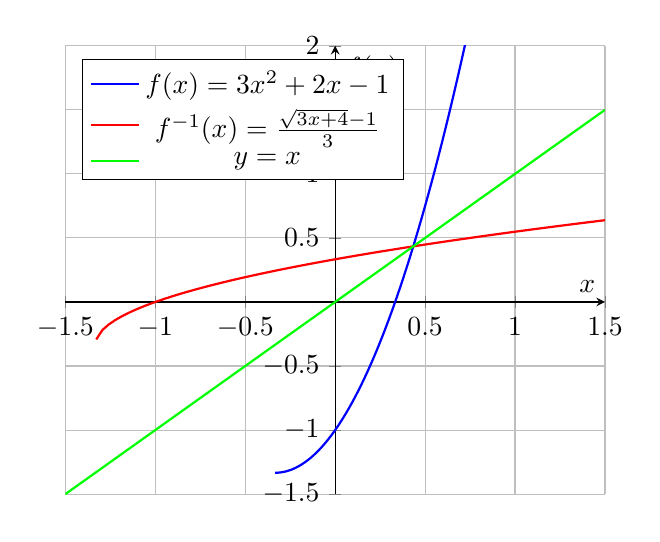
\begin{tikzpicture}
        \begin{axis}[
            axis lines = middle,
            xlabel = $x$, ylabel = {$f(x)$},
            xmin = -1.5, xmax = 1.5,
            ymin = -1.5, ymax = 2,
            xtick distance={0.5}, ytick distance={0.5},
            grid = both,
            legend pos = north west, % Positions the legend
        ]
            \addplot[blue, thick, domain=-0.33333:1.5, samples=100] {3 * x^2 + 2 * x - 1};
            \addlegendentry{$f(x) = 3x^{2}+2x-1$}

            \addplot[red, thick, domain=-2:1.5, samples=100] {(sqrt(3 * x + 4) - 1) / 3};
            \addlegendentry{$f^{-1}(x) = \frac{\sqrt{3x+4}-1}{3}$}

            \addplot[green, thick, domain=-2:1.5, samples=100] {x};
            \addlegendentry{$y = x$}
        \end{axis}
    \end{tikzpicture}
\end{figure}
\\
Now look at the graph for $f(x) = 3x^2 + 2x - 1$ and\\$f^{-1}(x) = \frac{-1 - \sqrt{3x + 4}}{3}$.
\vspace{-0.55cm}
\begin{figure}[ht]
    \centering
    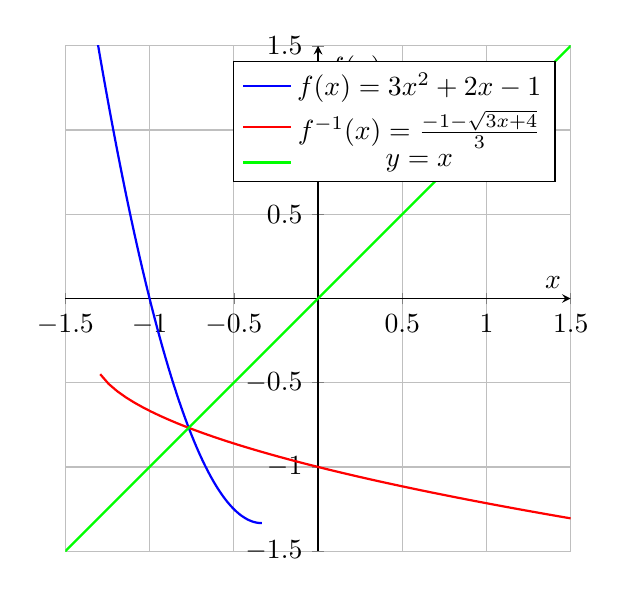
\begin{tikzpicture}
        \begin{axis}[
            axis lines = middle,
            xlabel = $x$, ylabel = {$f(x)$},
            xmin = -1.5, xmax = 1.5,
            ymin = -1.5, ymax = 1.5,
            xtick distance={0.5}, ytick distance={0.5},
            width = 8cm, height = 8cm,
            grid = both,
            legend pos = north east, % Positions the legend
        ]
            \addplot[blue, thick, domain=-2:-0.333333, samples=100] {3 * x^2 + 2 * x - 1};
            \addlegendentry{$f(x) = 3x^{2}+2x-1$}

            \addplot[red, thick, domain=-2:3, samples=100] {(-1 - sqrt(3 * x + 4)) / 3};
            \addlegendentry{$f^{-1}(x) = \frac{-1 - \sqrt{3x + 4}}{3}$}

            \addplot[green, thick, domain=-2:3, samples=100] {x};
            \addlegendentry{$y = x$}
        \end{axis}
    \end{tikzpicture}
\end{figure}
\\
Notice how these are also symmetric about the line $y = x$. The only difference is that the intersection is in the third quadrant instead of the first.
\clearpage
Although both are equally valid, the reason we take the positive solution is purely because of convention. Mathematicians came across this problem a while ago and had to decide which they wanted to normalize. They chose the positive solution as the convention, so that's what we use now.

I urge you to stick with the convention. Using the negative solution might not fare super well with your teacher (i.e. you may lose points for not choosing the positive).

As promised, I'll now give a probelm for you to try.
\begin{problem}
    Given the function $g(x) = \frac{3}{2x + 1}$, find the inverse function $g^{-1}$ and state its domain.
\end{problem}
\begin{solution}
    First, let's rewrite this function as an equation of $y$ in terms of $x$.
    \[
        y = \frac{3}{2x + 1}
    \]
    Next, let's swap the variables.
    \[
        x = \frac{3}{2y + 1}
    \]
    Now, let's solve for $y$.
    \begin{align*}
        x(2y + 1) &= 3 &&\text{Multiplied both sides by $2y + 1$} \\
        2y + 1 &= \frac{3}{x} && \text{Divided both sides by $x$} \\
        2y &= \frac{3}{x} - 1 && \text{Subtrated both sides by $1$} \\
        y &= \frac{\frac{3}{x} - 1}{2} && \text{Divided both sides by $2$}
    \end{align*}
    Since the denominator at the very bottom ($2$) doesn't have any variables, I can distribute it into the numerator. Doing so gives your inverse function.
    \[
        g^{-1}(x) = \frac{3}{2x} - \frac{1}{2}
    \]
    \clearpage
    Now to find the inverse. The only limitation here is the denominator $2x$. Since that denominator cannot equal $0$, we can set it equal to $0$ to see what value of $x$ would make the fraction invalid.
    \begin{align*}
        2x &= 0 \\
        x &= 0 && \text{Divided both sides by $2$}
    \end{align*}
    Although, we could've just noticed that anything times $0$ is $0$, meaning $2x = 0$ would simplify to $x = 0$, without doing any of that work. Since this is as simplified as it gets, we have our final answer:
    \[
        g^{-1}(x) = \frac{3}{2x} - \frac{1}{2} \text{ where } x \neq 0
    \]
\end{solution}